\documentclass{article}

% set font encoding for PDFLaTeX or XeLaTeX
\usepackage{ifxetex}
\ifxetex
  \usepackage{fontspec}
\else
  \usepackage[T1]{fontenc}
  \usepackage[utf8]{inputenc}
  \usepackage{lmodern}
  \usepackage{graphicx}
  \usepackage{siunitx}


\fi

% used in maketitle
\title{Atmosfera de la Tierra}
\usepackage[left=3cm,right=3cm,top=3cm,bottom=3cm]{geometry}
\author{Luis Aarón Cerón Ramírez}
\date{30 de enero,2017}

% Enable SageTeX to run SageMath code right inside this LaTeX file.
% documentation: http://mirrors.ctan.org/macros/latex/contrib/sagetex/sagetexpackage.pdf
% \usepackage{sagetex}

\begin{document}
\maketitle
\section{Introducción}
La atmósfera es un manto de gases, conocido como aire, el cual rodea la superficie terreste. Gracias a la atmósfera se tienen las condiciones necesarias para la creación y supevivencia de los seres vivos.
\newline
La atmósfera se compone por 20.95\% de oxigeno, 78.09\% de nitrogeno, 0.93\% de argón, 0.04 dióxido de carbono y pequeñas cantidades de gases.
\newline
Se pueden distiguir varias capas en la atmósfera, las cuales tienen sus propias caracteristicas, las cuales dependen de la altura y la temperatura.
\newline
El estudio de la atmósfera terrestre y sus procesos son estudiados por la ciencia atmósferica, en la cual entre sus pioneros se encuentran León Teisserenc de Bort y Richard Assmann.

\begin{figure}
  \centering
  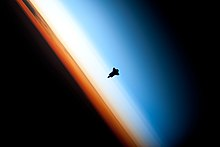
\includegraphics[scale=0.7]{at.jpg}
  \caption{Vista de las diferentes capas de la atmosfera }
  \label{fig:capas atmosferica}
\end{figure}

\section{Estructura de la atmósfera}
La presión y la densidad del aire decrecen con la altitud, la temperatura de la atmósfera terrestre varia con la altitud y es distinta dependiendo de la capa atmósferica en la que se este, la atmosfera esta dividida en 5 capas principales.
\newline
La atmosfera esta compuesta principalmente por los compuestos que se presentan en la siguiente tabla.

\begin{table}[htp]
\centering
\begin{tabular}{|c|c|c|c|}
\hline
Nombre & Formula & en ppmv & Porcentaje \\ \hline
nitrógeno & $N_2$ & 780.840 & 78.084\% \\ \hline
oxígeno & $O_2$ & 209.460 & 20.946\% \\ \hline
argón & Ar & 9.340 & 0.934\% \\ \hline
dióxido de carbono & $CO_2$ & 400 & 0.04\% \\ \hline
neón & Ne & 18.18 & 0.001818\% \\ \hline
helio & He & 5.24 & 0.000524\% \\ \hline
metano & $CH_4$ & 1.79 & 0.000179\% \\ \hline

\end{tabular}
\caption{Tabla de valores}
\label{Tabla 1}
\end{table}

\subsection{Exosfera}
La exosfera es la capa mas externa de la atmósfera terrestre, esta se extiende de la exobase la cual se extiende en la parte superior de la termosfera a una altitud de unos 700 km sobre el nivel del mar.
\newline
Esta capa esta compuesta principalmente por hidrogeno de baja densidad, helio y varias moleculas pesadas como nitrogeno, oxigeno y dioxido de carbono.
\newline
Esta capa al encontrarse muy por encima de la superficie terrestre provoca que no forme ningun fenomeno meteorologico, aunque la aurora borealis y aurora austrialis pueden ser observada en la parte mas baja de esta.
\newline
Es en la exosfera donde se encuentra la mayoria de los satélites orbitando.

\subsection{Termosfera}
La termosfera es la segunda capa mas alta de la atmósfera terrestre, esta se extiende desde la mesopausa \footnote {mesopausa: \textit{zona de la atmósfera terrestre que sirve como limite entre la mesosfera y la ionesfera}} a una altitud de 80 km hasta la termopausa\footnote {termopausa:\textit{zona de la atmosfera terrestre que sirve de limite entre la ionosfera y la exosfera}} que se encuentra en una altitud de entre 500- 1000 km.
\newline
Es en esta capa donde la radiacion ultravioleta y especialmente los rayos gammas y los rayos x que origina el sol , causan una constente ionizacion de los gases que la componen, esta eleva su temperatura varios cientos de grados lo que le da su nombre.
\newline
ESta capa esta completamente libre de nubes y vapor de agua , sin embargo ocasionalmente pueden ser observadas auroras borialis y auroras australis.

\subsection{Mesosfera}
Esta es la parte de la atmósfera que se encuentra entre la termosfera y la estratosfera.En esta capa la temperatura va disminuyendo a medida que la temeratura aumentahasta llegar a los $80^{\circ}$C a los 80 km aproximadamente.
\newline
En este pubnto la temperatura es tan baja que el vapor de agua puede formaar escarcha de hielo, en esta zona es donde se encuentran las nubes mas altas.

\subsection{Estratosfera}
Esta es la segunda capa mas baja, esta se encuentra por encima de la troposferay es separadade esta por la tropopausa\footnote {termopausa:\textit{zona de la atmósfera terrestre que sirve de límite entre la troposfera y la estratosfera.}}, la estratosfera se encuentra a una altura de unos 10-15 km de altura y se extiende hasta unos 45-50 km. La temperatura en la estratosfera va variando de la siguiente manera, comienza siendo estable (ya que se encuentra en alturas cercanas a la tropopausa donde la temperatura se mantiene igual) y bastante baja. Conforme vamos aumentando en altitud, la temperatura de la estratosfera va aumentando, ya que va absorbiendo cada vez más cantidad de radiación solar. El comportamiento de la temperatura en la troposfera funciona al contrario de lo que lo hace la troposfera en la que vivimos, es decir, en vez de decrecer con la altura, aumenta.

\subsection{Troposfera}
Es la capa más baja de la atmósfera terrestre, sede de los fenómenos meteorológicos. Se extiende desde el nivel del suelo hasta 11 km de altura y está carecterizada por temperaturas decrecientes del orden de $6^{\circ}$C por km.
\newline
La parte mas baja de la tropsfera es normalmente la mas calida de esta. Esta capa contiene el 80\% de la masa de la atmosfera terrestre, ademas de ser la mas densa de las capas gracias a la compresion provocada por las demas al ser la mas baja el 15\% de la masa total de está, esta localizadapor debajo de los 5.7 km.

\section{Propiedades fisicas}
\subsection{Presión y espesor}
La presion atmosferica promedio a nivel del mar es de aproximadamente de 101325 Pa, la cual es conocida como la unidad estandar.
\newline
La presion atmosferica es el peso total del aire sobre unidad de área en el punto donde esta se mide, es por esta razon que al no ser uniforme la Tierra, hace que varie la presión.
\newline
Si toda la masa de la atmósfera tuviera una densidad uniforme desde el nivel del mar, terminaría abruptamente a una altitud de 8,50 km (27,900 pies). En realidad, disminuye exponencialmente con la altitud, cayendo a la mitad cada 5,6 km (18.000 pies) o por un factor de 1 / e cada 7,64 kilometros (25.100 pies), la altura promedio de la escala de la atmósfera por debajo de 70 km (43 mi; 230.000 pies).
\newline
En resumen, la masa de la atmósfera de la Tierra se distribuye aproximadamente de la siguiente manera:
\newline
está por debajo de 5.6 km (18,000 pies).
\newline
está por debajo de 16 km (52,000 pies).
\newline
99.99997\% está por debajo de 100 km (62 mi; 330,000 pies), la línea Kármán. Según una convención internacional, esto marca el comienzo del espacio donde los viajeros humanos son considerados astronautas.

\subsection{Temperatura y velocidad del sonido}
La temperatura disminuye con la altitud comenzando al nivel del mar, pero las variaciones en esta tendencia comienzan por encima de los 11 km, donde la temperatura se estabiliza a través de una gran distancia vertical a través del resto de la troposfera. En la estratosfera, comenzando por encima de unos 20 km, la temperatura aumenta con la altura, debido al calentamiento dentro de la capa de ozono causado por la captura de radiación ultravioleta significativa del Sol por el dioxígeno y el gas ozono en esta región.
\newline
Debido a que en un gas ideal de composición constante, la velocidad del sonido depende únicamente de la temperatura y no de la presión o densidad del gas, la velocidad del sonido en la atmósfera con la altitud adquiere la forma del perfil de temperatura complicado y no refleja los cambios altitudinales en densidad o presión.

\begin{figure}
  \centering
  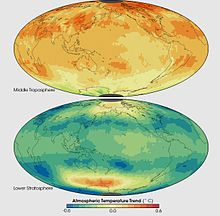
\includegraphics[scale=0.35]{temperatura.jpg}
  \caption{Tendencias de temperatura en dos capas gruesas de la atmósfera, medidas entre enero de 1979 y diciembre de 2005  }
  \label{fig:Temperatura}
\end{figure}

\subsection{Densidad y masa}
La densidad del aire a nivel del mar es de aproximadamente 1.2 kg / $m^3$ (1.2 g / L, 0.0012 g /$cm^3$).
La densidad no se mide directamente, pero se calcula a partir de mediciones de temperatura, presión y humedad utilizando la ecuación de estado para el aire (una forma de la ley de los gases ideales). La densidad atmosférica disminuye a medida que aumenta la altitud.
\newline
Según el Centro Nacional Americano de Investigación Atmosférica, "La masa media total de la atmósfera es 5.1480\num{1e18}kg con un rango anual debido al vapor de agua de 1.2 o 1.5 \num{1e15} kg, dependiendo de si se usan datos de presión superficial o vapor de agua algo más pequeña que la estimación anterior. La masa media de vapor de agua se estima en 1.27\num{1e16}kg y la masa de aire seco en $5.1352 \pm 0.0003\num{1e18}$kg.

\section{Propiedades opticas}
La mayor parte de la energía que llega a nuestro planeta procede del Sol. El Sol emite energía en forma de radiación electromagnética. Estas radiaciones se distinguen por sus diferentes longitudes de onda. Algunas, como las ondas de radio, llegan a tener longitudes de onda de kilómetros, mientras que las más energéticas, como los rayos X o las radiaciones gamma, tienen longitudes de onda de milésimas de nanómetro.
\newline
La radiación en el Sol es de 63 450 720 ${W/m^2}$. La energía que llega al exterior de la atmósfera terrestre sobre una superficie perpendicular a los rayos solares lo hace en una cantidad fija, llamada constante solar  variable durante el año un 3\% a causa de la elipticidad de la órbita terrestre.
\newline
Esta energía es una mezcla de radiaciones de longitudes de onda entre 200 nm y 4000 nm, que se distingue entre radiación ultravioleta, luz visible y radiación infrarroja.

\subsection{Dispersión}
Es una difusión de la radiación producida por partículas de la atmósfera y podemos  considerar tres mecanismos principales: dispersión de Rayleigh, dispersión de Mie y  dispersión no selectiva. La dispersión de Rayleigh es consecuencia de la interacción de la radiación con moléculas  de los gases atmosféricos y con otras partículas pequeñas de diámetro mucho menor que
la longitud de onda de la radiación con la que interaccionan. Este efecto es inversamente  proporcional a la 4ta potencia de la longitud de onda.
\newline
La dispersión no selectiva constituye un fenómeno mucho más molesto que los anteriores y se produce cuando los diámetros de las partículas que producen la dispersión son mucho mayores que las longitudes de onda con que interaccionan.
\newline
 La dispersión de Mie se produce cuando los diámetros de las partículas atmosféricas son esencialmente iguales a la longitud de onda de la radiación (vapor de agua, polvo fino, etc.) y tiende a influenciar la radiación de longitudes de onda mayores que las afectadas por la dispersión de Rayleigh.

\subsection{Absorción}
Contrariamente a lo que ocurre en la dispersión, en la absorción se produce una transferencia de energía de la radiación a los constituyentes atmosféricos. Este mecanismo implica absorción de energía de determinada o determinadas longitudes de onda. Desde este punto de vista los absorbentes más eficaces de radiación solar son las moléculas de agua, de dióxido de carbono y ozono. La absorción selectiva de ciertas longitudes de onda por estas moléculas hace que la atmósfera constituya un medio opaco para ciertos rangos espectrales, mientras que ofrezca ventanas libres de absorción para otros rangos. A través de dichas ventanas deben mirar los satélites de observación.

\begin{figure}
  \centering
  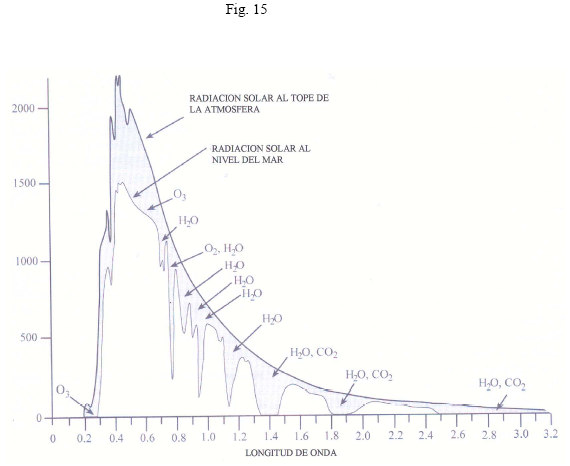
\includegraphics[scale=0.35]{absorcion.jpg}
  \caption{efectos combinados que diversos componentes atmosféricos ejercen sobre la radiación  electromagnética }
  \label{fig:absorcion}
\end{figure}

\subsection{Indice de refracción}
El índice de refracción del aire es cercano, pero apenas superior a 1. Las variaciones sistemáticas en el índice de refracción pueden conducir a la flexión de los rayos de luz en recorridos ópticos largos.
\newline
El índice de refracción del aire depende de la temperatura, dando lugar a efectos de refracción cuando el gradiente de temperatura es grande. Un ejemplo de tales efectos es el espejismo.

\subsection{Emisión}
El espectro de emisión atómica de un elemento es un conjunto de frecuencias de las ondas electromagnéticas emitidas por átomos de ese elemento, en estado gaseoso, cuando se le comunica energía. El espectro de emisión de cada elemento es único y puede ser usado para determinar si ese elemento es parte de un compuesto desconocido.


\section{Circulación}
La circulación atmosférica es el movimiento de aire a gran escala a través de la troposfera, y los medios (con circulación oceánica) por los cuales se distribuye el calor alrededor de la Tierra. La estructura a gran escala de la circulación atmosférica varía de un año a otro, pero la estructura básica permanece bastante constante porque está determinada por la velocidad de rotación de la Tierra y la diferencia en la radiación solar entre el ecuador y los polos.

\begin{figure}
  \centering
  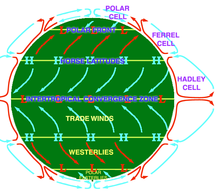
\includegraphics[scale=0.6]{circulacion.png}
  \caption{Una vista idealizada de tres celdas de gran circulación.}
  \label{fig:circulacion de la atmosfera}
\end{figure}

\section{Apendice}
1.- ¿Qué fue lo que más te llamó la atención de esta actividad?
\newline
El hecho de tener que buscar la informacion refernte al uso del latex la cual nos brindara los recursos para poder escribir
\newline
2.- ¿Qué fue lo que se te hizo menos interesante?
\newline
Mi unico problema con la actividad fue el hecho de tener que traducir el articulo de la wikipedia, pues en mi caso no domino del todo el ingles
\newline
3.- ¿Qué cambios harías para mejorar esta actividad?
\newline
Agregaria mas material para buscar sobre el tema en ingles y español ó hacer tema libre centrandoo en el uso de los comandos de latex
\newline
4.- ¿Cuál es tu primera impresión de uso de LATEX?
\newline
En un principio es complicado acostumbrarse a utilizarlo , pero despues se vuelve muas facil en parte a la gran cantidad de material que hay en internet
\newline
5.- ¿El tiempo sugerido para esta actividad fue suficiente?
si, en mi caso tuve algunas complicaciones con otras materias por lo que no pude subirla a tiempo pero el tiempo me parecio suficiente
\newline
6.- ¿Encontraste algún documento o recurso en línea útil que quisieras compartir con los demás?
\newline
Encontre varios recursos pero no me parece que sean lo suficientemente buenos como para compartirlos



\begin{thebibliography}{0}
\bibitem {Wikipedia} Atmosphere of Earth. (2018, January 29). In Wikipedia, The Free Encyclopedia. Retrieved 19:36, February 12, 2018
\end{thebibliography}


\end{document}


